\documentclass[11pt]{jarticle} 

\usepackage[dvipdfmx]{graphicx} % 画像を使うためのパッケージ
\usepackage{amsmath, amsfonts} % 数式を使うためのパッケージ
\usepackage{bm} % 太字の数式を使う
\usepackage{fancyhdr}
\usepackage{wrapfig} %図に対して文章をを回り込ませるfigure

\setlength{\oddsidemargin}{-10mm} % 紙の左のマージン
\setlength{\evensidemargin}{-10mm} % 紙の右のマージン
\setlength{\textwidth}{180mm} % テキストの幅 を指定

\setlength{\topmargin}{-15mm} % 紙の上のマージン
\setlength{\textheight}{255mm} % テキストの高さ

\lhead{東京科学大学 卒業論文中間報告書} %ヘッダ左
\chead{\empty} %ヘッダ中央
\rhead{提出日:2025年8月1日} %ヘッダ右.コンパイルした日付を表示
\lfoot{\empty} %フッタ左
\cfoot{\thepage} %フッタ中央.ページ番号を表示
\rfoot{\empty} %フッタ右

\pagestyle{fancy}

% 図とキャプションの間のスペースを調節
\setlength\abovecaptionskip{0pt}

% 図と図の間のスペースを調節
% \setlength\floatsep{0pt}

% ページの上下に表示される図と本文の間のスペースを調節
% \setlength\textfloatsep{0pt}

% ページの途中に表示される図と本文の間のスペースを調節
\setlength\intextsep{0pt}

% ここから本文
\begin{document}

% --------------------------------------------------------

\title{研究題目}
\title{高効率な制御器導出のための\\On-the-fly直接導出による計算空間削減}
\author{都竹 佑季 (22B30490) \;\; 指導教員:鄭 顕志}
\date{\empty} % 日付は自動的に今日の日付が入る
\maketitle % 上で指定した title と authorを出力
\thispagestyle{fancy}

% --------------------------------------------------------

\section{概要} % \section, \subsection, \subsubsection
本研究では,制御効率の高い制御器の導出における計算空間の爆発の課題に対処するため,On-the-fly探索を用いた制御器の直接合成手法を提案する.
On-the-fly探索は,動作仕様を満たす目標状態への状態遷移を逐次的に構築するため,制御効率を指標として非効率な状態構築を排除しつつ探索することで,従来構築されていた非効率な制御の構築を回避することができる.
本研究では,このOn-the-fly探索を制御効率の考慮した制御器合成分野に拡張し,計算空間削減を図る.

\section{スーパーバイザ制御のための制御効率の良い制御器の設計}
% 離散事象システム
離散事象システムとは,離散的な状態集合を持ち,事象の発生によって状態が変化する事象駆動型のシステムの総称である.通信システム,オペレーティングシステム,データベースシステム,生産システム,交通システムなど,さまざまな分野のシステムがこの性質を備えている.

% スーパーバイザ制御
離散事象システムを安全かつ信頼性の高い形で運用するためには,安全性,到達可能性といった制御仕様を確実に満たすことが求められる.この課題に対し,スーパーバイザ制御と呼ばれる手法が広く研究されてきた.

スーパーバイザ制御は,動作仕様の充足が保証された制御器に基づいてシステムを制御することで,その振る舞いが常に制御仕様を満たすように導く制御手法である.この手法では,まず開発者が,実際のシステムが運用される動作環境を形式的にモデル化し,Labelled Transition System(LTS)として表現する.これは,制御対象となるシステムと,システムに関与するすべての環境の振る舞いを,状態遷移モデルであるLTSで明示的に記述する.
次に,この環境の中で保証すべき安全性や到達可能性などの制御仕様を定義し,それを監視するための監視モデルを,同様にLTSとして構築する.
こうして得られた環境モデルと監視モデルを入力とし,制御仕様が満たされるか否かを検証するためのゲーム空間を並列合成を用いて自動構成する.
その後,構築されたゲーム空間において二人型対戦ゲームを解くことによって,制御器と呼ばれる動作仕様が保証される環境モデル上の全状態空間が導出される.
このようにして合成された制御器に基づいてシステムをスーパーバイザ制御することで,システムの振る舞いにおいて安全性を保証することが可能となる.

一方で,制御器上で選択する制御の内容によっては,実行時間や実行料金といったシステムの性能に差異が生じる.
このため,スーパーバイザ制御においては,システム上で発生する各事象に対応する実行コストを考慮して,制御器から非効率な制御を排除した制御効率の良い制御器を導出する研究が進められてきた\cite{eze}.

% --------------------------------------------------------

\section{制御器の合成における課題}
しかし,制御器の導出過程で構築されるゲーム空間は指数関数的に増加する課題があり,スーパーバイザ制御を実践的な規模のシステム開発への適用を困難にしている.
ゲーム空間は,事象の同期を考慮した環境モデルと監視モデルの全状態の直積により状態を構築するため,各モデル数の増加に伴って状態数が指数関数的に増加する.
このゲーム空間の指数関数的増加に伴って,要求される計算空間,計算時間,必要主記憶量も指数関数的に増加するため,制御器を導出するにあたって計算空間の状態削減は重要な課題となっている.

% --------------------------------------------------------

\section{実行コストを考慮したOn-the-fly制御器導出手法}
本研究では,制御器導出過程における計算空間爆発の問題に対処するため,On-the-fly探索を用いて制御効率を考慮した制御器の直接合成に取り組む.

On-the-fly探索\cite{ddcs}は,環境モデルと監視モデルに加え,目標状態が与えられた上で,動作仕様を違反しない状態遷移を初期状態から目標状態に向けて逐次的に探索・構築する手法である.本手法では,動作仕様を満たす目標状態への状態遷移がひとつでも見つかれば探索を終了するため,ゲーム空間全体を網羅的に構築・探索する必要がない.
このような性質により,On-the-fly探索に基づく制御器の導出は,計算空間を大幅に削減できるという利点がある.一方で,目標状態に到達する経路がひとつだけ導出されるため,探索方針に依存して制御器の内容が変化するという欠点がある.

そこで本研究では,各事象に対する実行コストを考慮しつつOn-the-fly探索を実行することで,環境モデル・監視モデル・実行コストの情報から,制御効率の高い制御器を直接導出する.このような制御効率を指標とした制御器の導出において,On-the-fly探索は従来扱われてこなかった.On-the-fly探索の「ひとつの制御のみ導出する」という欠点は,状態空間削減の観点で見ると制御効率の低い状態と遷移の構築を避けられるため,本研究では積極的に活用し,制御器の導出における計算空間の爆発の課題に対処する.

\begin{figure}[h]
  \centering
  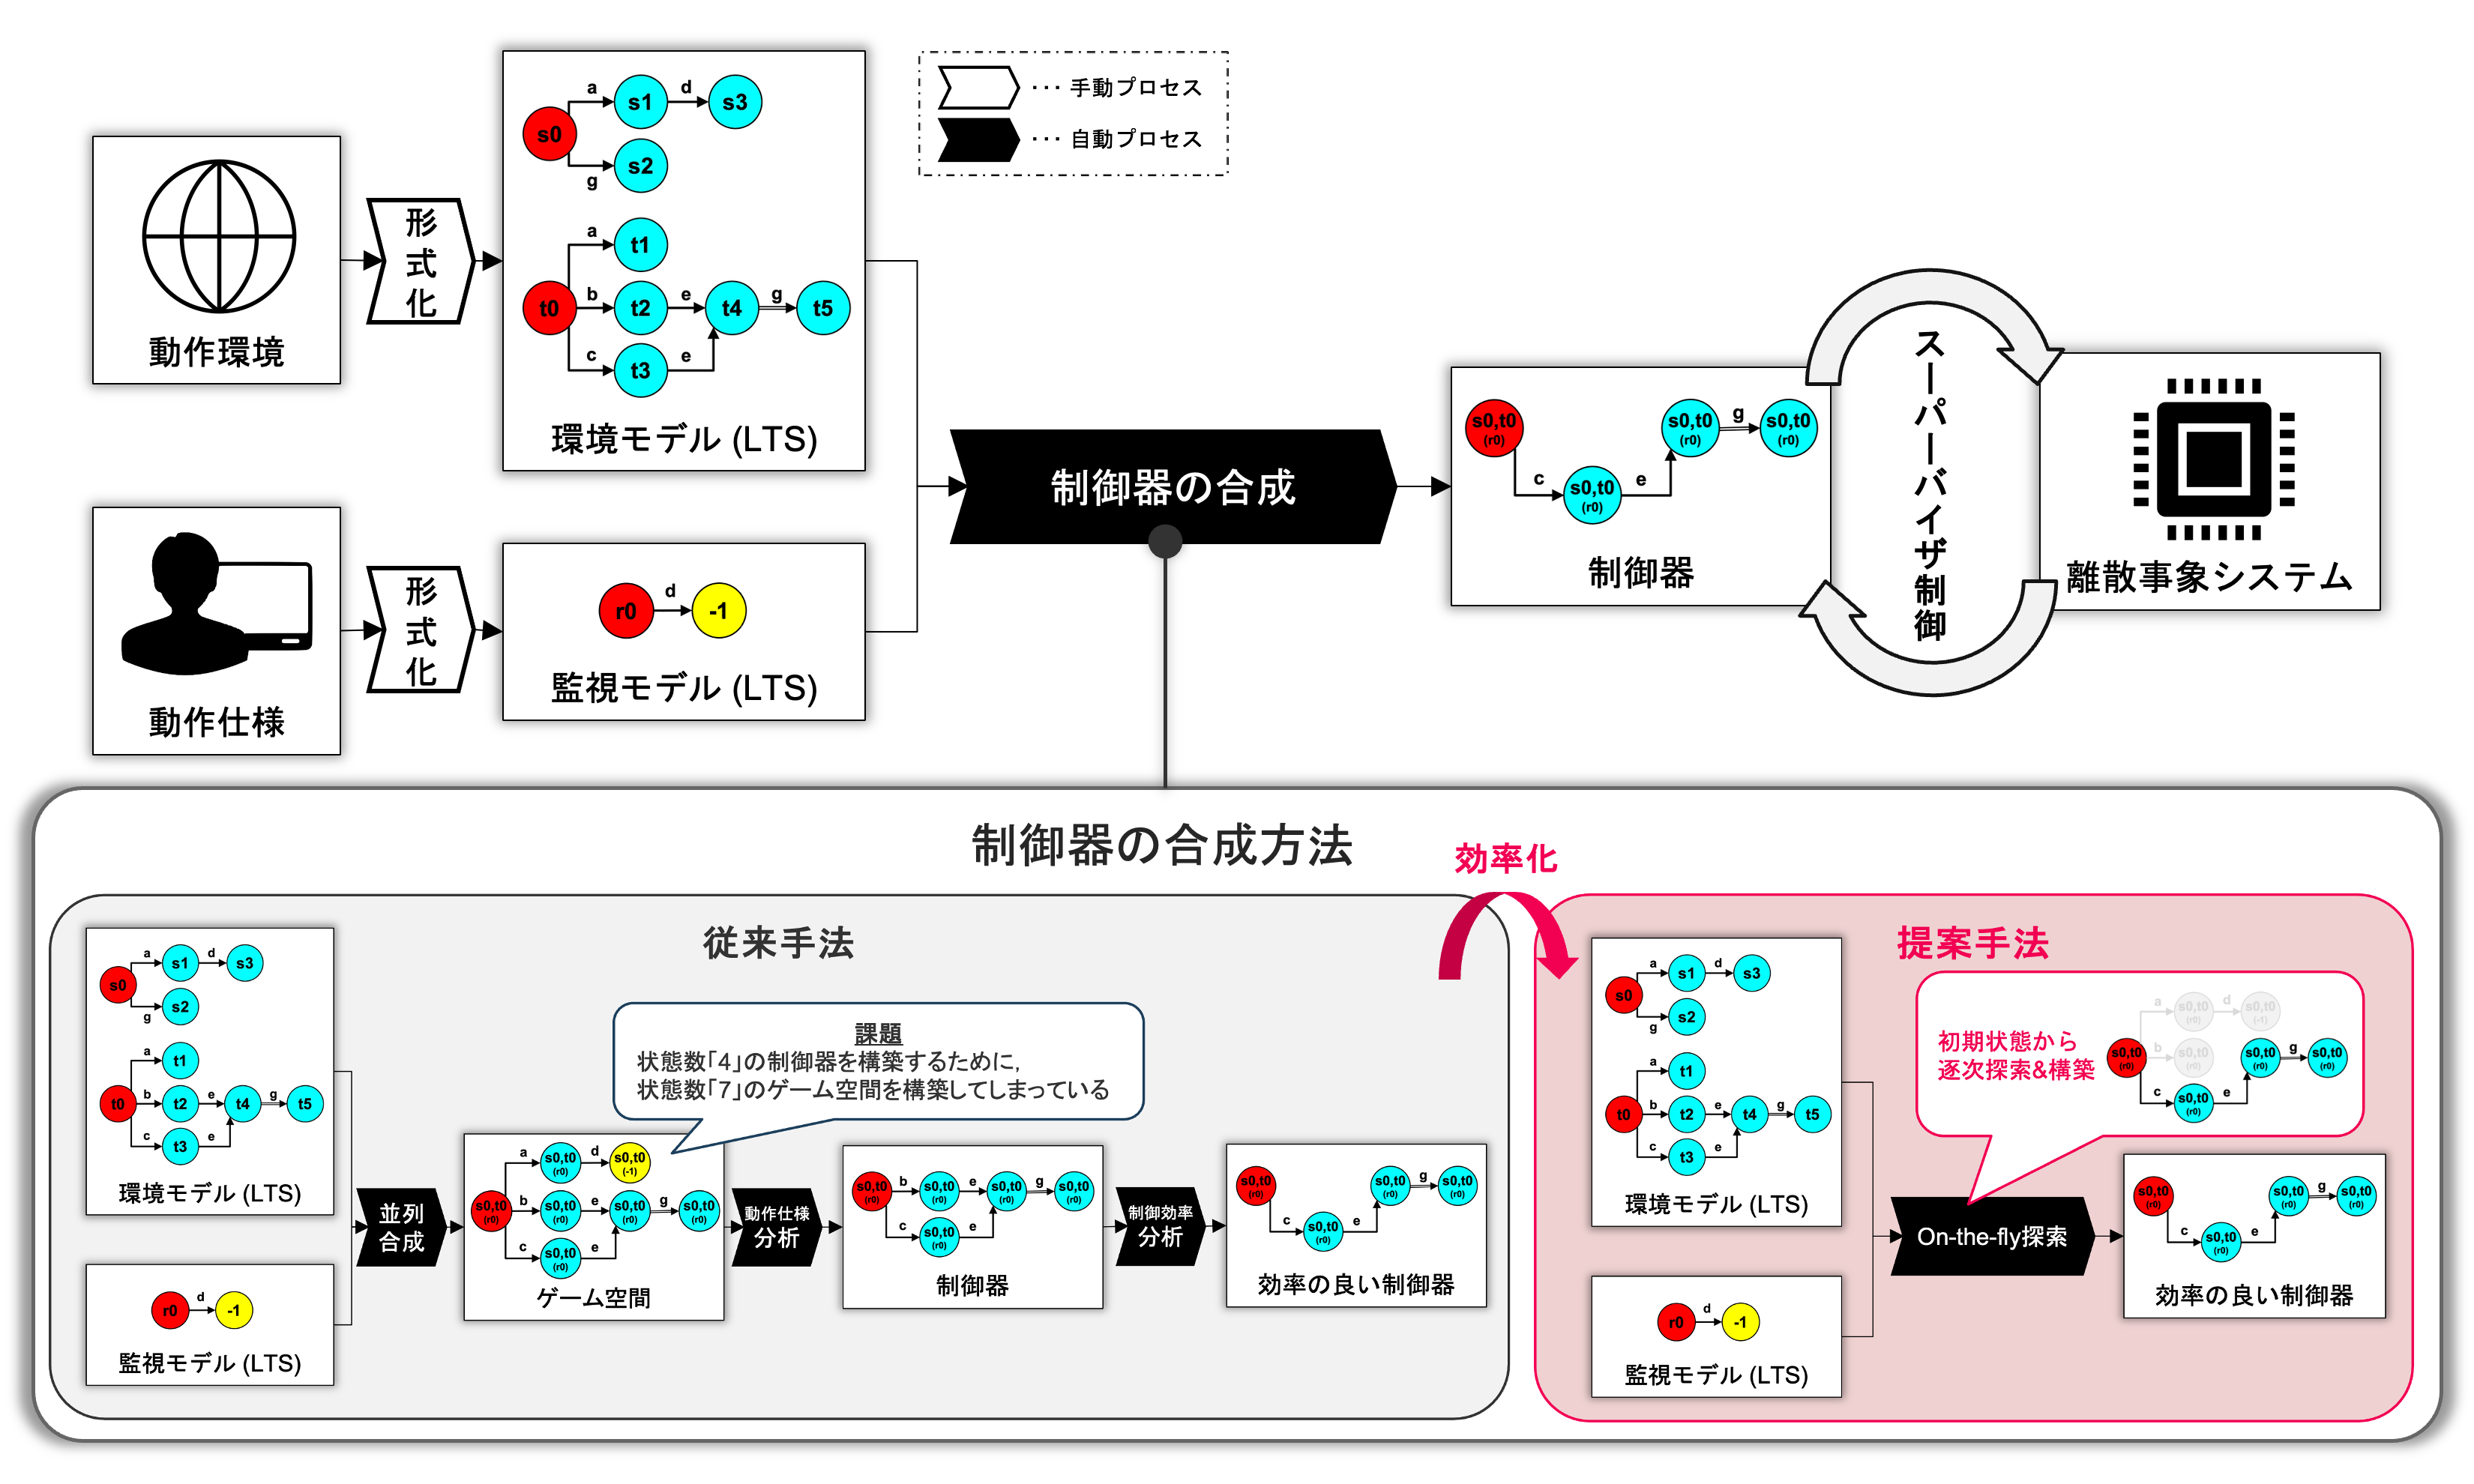
\includegraphics[width=16cm]{./figures/proposal.png}
  \caption{スーパーバイザ制御における制御器導出方法(従来手法と提案手法)の比較}
  \label{fig:3}
\end{figure}

% --------------------------------------------------------

\section{研究計画}
現在までに,提案手法の実装は概ね完了している.
今後は,8月中に本手法の有効性を検証するための評価実験を実施する予定である.
評価結果をもとに,9月にはソフトウェア工学分野の研究会であるSIG-KBSEへの論文投稿を目指す.
論文が採択された場合,11月に開催される同研究会において研究成果の発表を行う.
12月から翌年1月にかけては,これまでの研究内容を取りまとめ,卒業論文の執筆を進める計画である.

% --------------------------------------------------------

\begin{thebibliography}{99} % 文献リスト一覧はこんな風に始める
{\footnotesize

\bibitem{eze} % bibitem でラベルを付けて
E. Castellano, V. Braberman, N. D'Ippolito, S. Uchitel, and K. Tei, 
Minimising Makespan of Discrete Controllers: A Qualitative Approach,
in 2019 IEEE 58th
Conference on Decision and Control (CDC), Nice, France, 2019, pp. 1068-1075..

\bibitem{ddcs} % bibitem でラベルを付けて
D. Ciolek, M. Duran, F. Zanollo, N. Pazos, J. Braier, V. Braberman, N. D'Ippolito, and S.
Uchitel, On-the-fly informed search of non-blocking directed controllers,
Automatica, vol. 147, No. C (2023).

}
\end{thebibliography} % 文献リストの最後に必要

% --------------------------------------------------------

\end{document} % 最後の締めくくり.絶体必要